\section{Experiment system}
\label{sec:system}

In this section, we describe Mira - an IBM Glue Gene Q supercomputer in which we developed our algorithms and a framework for network load balancing and conducted our experiments. The Argonne Leadership Computing Facility (ALCF) maintains several compute-analysis systems used by the scientific community. Figure \ref{fig:alcf} depicts the architecture of the primary ALCF resources, consisting of the Blue Gene/Q compute cluster (Mira), the data analysis cluster (Tukey), and the file server nodes.

\begin{figure}[!htb]
\vspace{-0.1in}
\centering
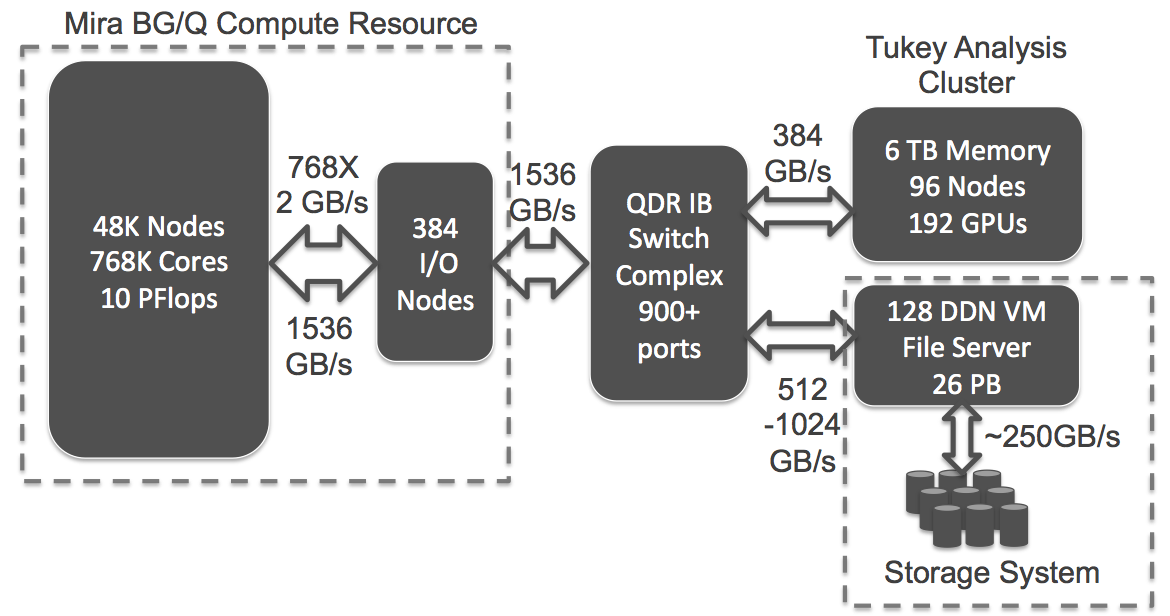
\includegraphics[scale=0.2]{figures/anl_facility}
\vspace{-0.1in}
\caption{The ALCF maintains the 768K core Blue Gene/Q compute cluster (Mira), data analysis cluster (Tukey), and file server nodes.}
\vspace{-0.1in}
\label{fig:alcf}
\end{figure}


Mira \cite{Chen:BGQ}, with 48 compute racks (48K nodes and 768K cores) at the ALCF, provides 10 PFlops theoretical peak performance. Each node has a 16-core processor and 16 GB of memory.

The interprocess communications of Blue Gene/Q travel on a 5D torus network both for point-to-point and for collective communications. This 5D torus interconnects a compute node with its 10 neighbors at 2 GB/s theoretical peak over each link in each direction, making a total of 40 GB/s bandwidth in both directions for a single compute node. Because of packet and protocol overheads, however, only up to 90\% of the raw data rate (1.8 GB/s) is available for user data. The machine can be partitioned into non-overlapping rectangular submachines; these submachines do not interfere with each other except for I/O nodes and the corresponding storage system.

For interconnect network traffic, BG/Q supports both deterministic and dynamic routing \cite{Chen:BGQ}. In deterministic routing, packets are routed based on dimension-ordered routing, from the longest first to the shortest last. In dynamic routing, routing is still dimension-ordered, but it is programmable, enabling different routing algorithms to be used. Given the size of a certain message, routing is always the same, and its path is known before it is routed. These are the default routing algorithms and cannot be changed during run time. However, one can set which routing zone id to use by using the PAMI\_ROUTING environment variable. Since BG/Q uses single-path data routing, for sending/receiving a message only one link of the ten available is used. The details of routing can be found in \cite{Chen:BGQ}.

PAMI is a low-level communication library for BG/Q \cite{PAMI:Kumar}. PAMI provides low-overhead communication by using various techniques such as accelerating communication using threads, scalable atomic primitives, and lockless algorithms to increase the messaging rate. Since MPI is implemented on top of PAMI, direct use of PAMI would provide higher messaging rates as well as lower latencies in comparison with MPI.


